% 本文件是示例论文的一部分
% 论文的主文件位于上级目录的 `main.tex`
\chapter{检测系统的设计与实现}

\section{需求分析}
该系统需要为用户提供头盔佩戴情况检测和历史检测数据查询两个功能,本文为这两个功能各自设计并实现了前端页面。检测页面允许用户上传待检测图片、静态视频文件和实时监控视频,并需要支持用户自定义检测模型、IoU和置信度参数。后端接收到参数之后调用模型进行头盔佩戴情况检测,并返回检测结果给前端。查询页面可供用户查询历史检测记录,允许用户对驾驶员、检测时间、检测地点等字段进行过滤。通过可视化图表展示查询结果,便于用户进行数据分析。

\section{系统整体架构}
\begin{figure}[!htb]
    \centering
    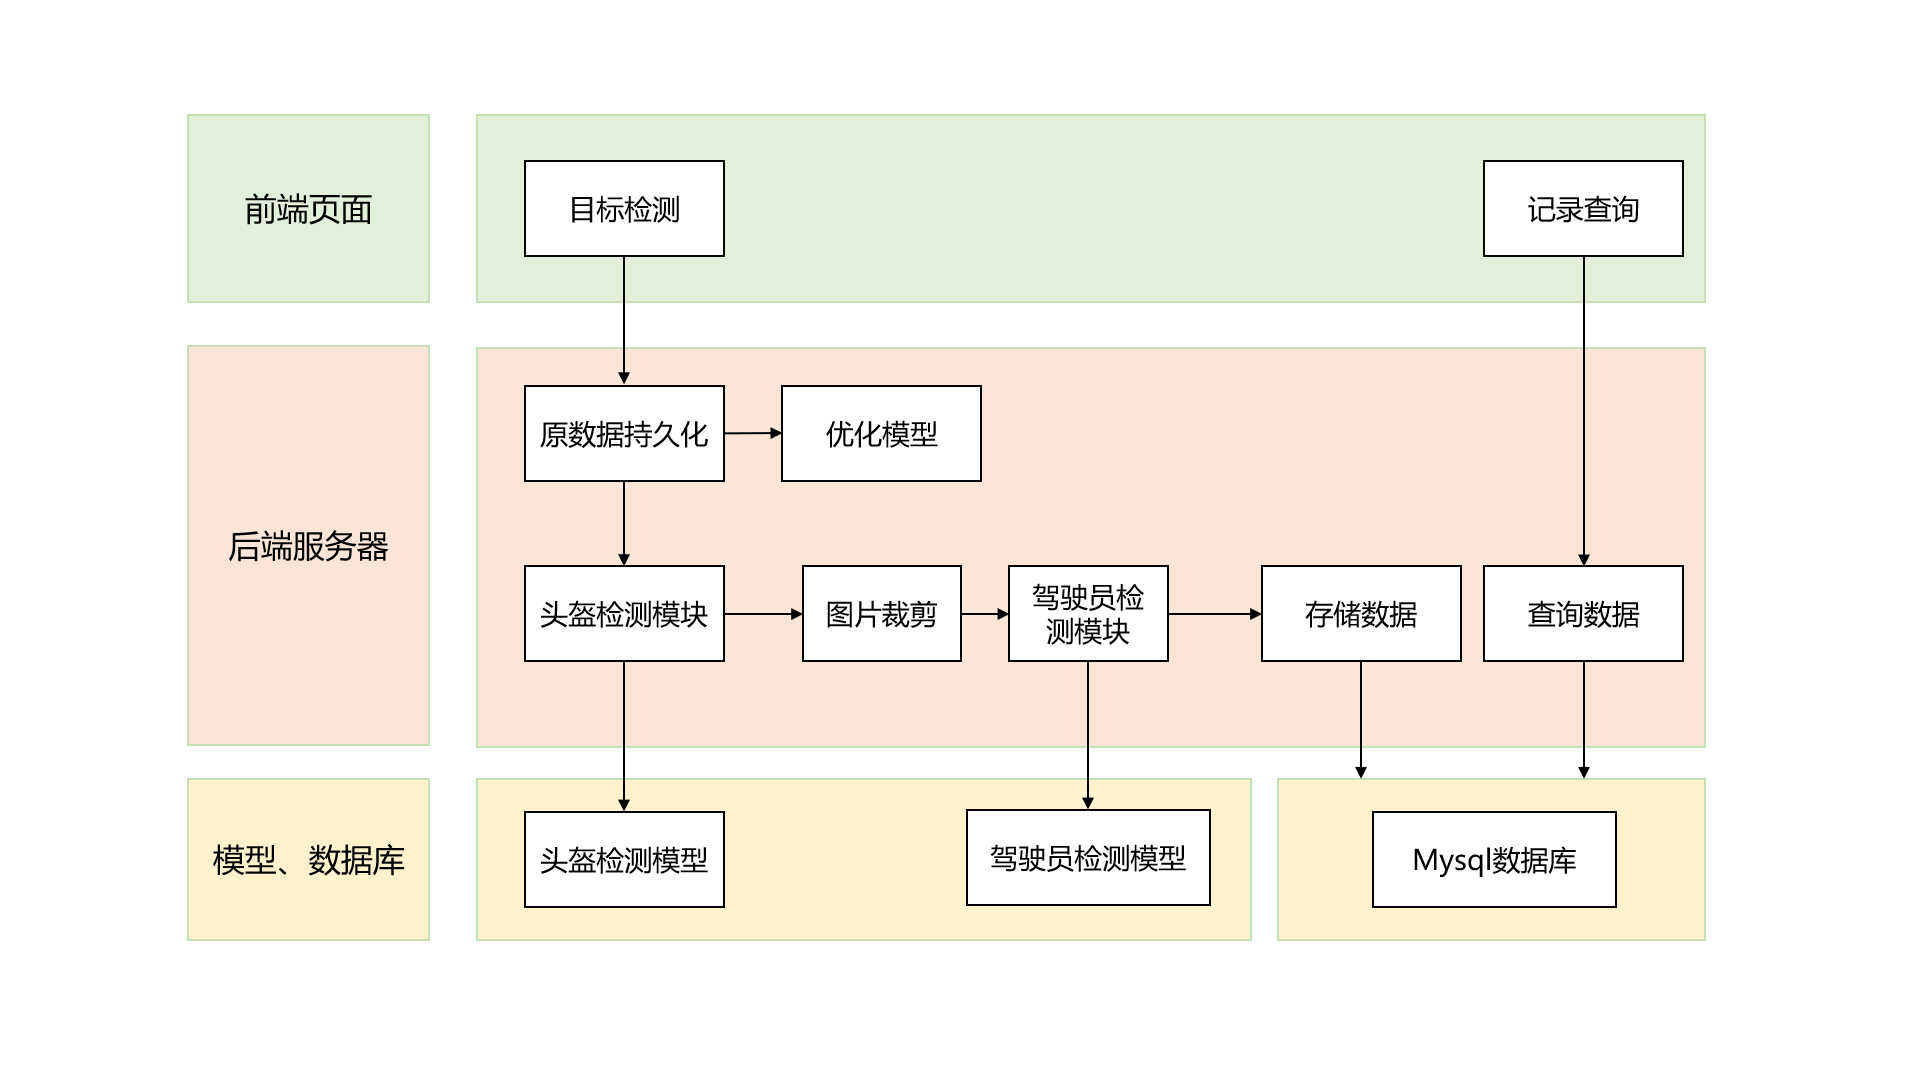
\includegraphics[width=1\textwidth]{figs/chap05/struct.png}
    \caption{系统架构图}
    \label{fig:struct}
\end{figure}
本系统整体架构如\ref{fig:struct}所示。本系统前端为用户提供目标检测和记录查询功能。目标检测界面展示后端返回的带检测框的结果并提供保存功能;记录查询界面通过ECharts组件以柱状图、折线图和饼图可视化展示后端查询的历史数据。

后端处理目标检测请求时:先持久化检测原数据,用于后续优化模型;再将用户传入的自定义检测模型、IoU及置信度参数动态拼接到python脚本,调用训练好的头盔佩戴检测模型预测,并按边界框裁剪原数据;接着将裁剪图片作为驾驶员id检测模型的输入,检测驾驶员信息;最后把检测结果存至Mysql数据库,并将带检测框结果返回前端。处理记录查询请求时,根据前端传来的过滤条件动态拼接Sql语句查询数据库。

\section{前端模块设计与实现}
前端界面分为目标检测界面和记录查询界面。两个界面都以灰、蓝色为主题色调,并且背景以及各个功能区的CSS样式几乎一样,使得两个页面非常协调。
\subsection{目标检测界面}
% \subsubsection{界面设计与实现}
目标检测界面用例设计如\ref{fig:uml1}。核心用例为头盔佩戴检测,其包含上传待检测资源、选择模型,设置IOU和置信度、请求后端检测、浏览检测结果和保存检测结果五个子用例。
上传待检测资源包含上传视频和上传图片两个子用例,支持用户上传视频和图片资源。选择模型,设置IOU和置信度用例允许用户选择检测模型,自定义检测IOU和置信度阈值。请求后端检测用例会将待检测资源和用户设置参数上传至后端服务器请求头盔佩戴检测。检测结果浏览功能负责把检测所得结果展示在页面,并且提供保存功能,让用户可以把展示的检测结果保存至本地,实现数据的本地化存储。

\begin{figure}[!htb]
    \centering
    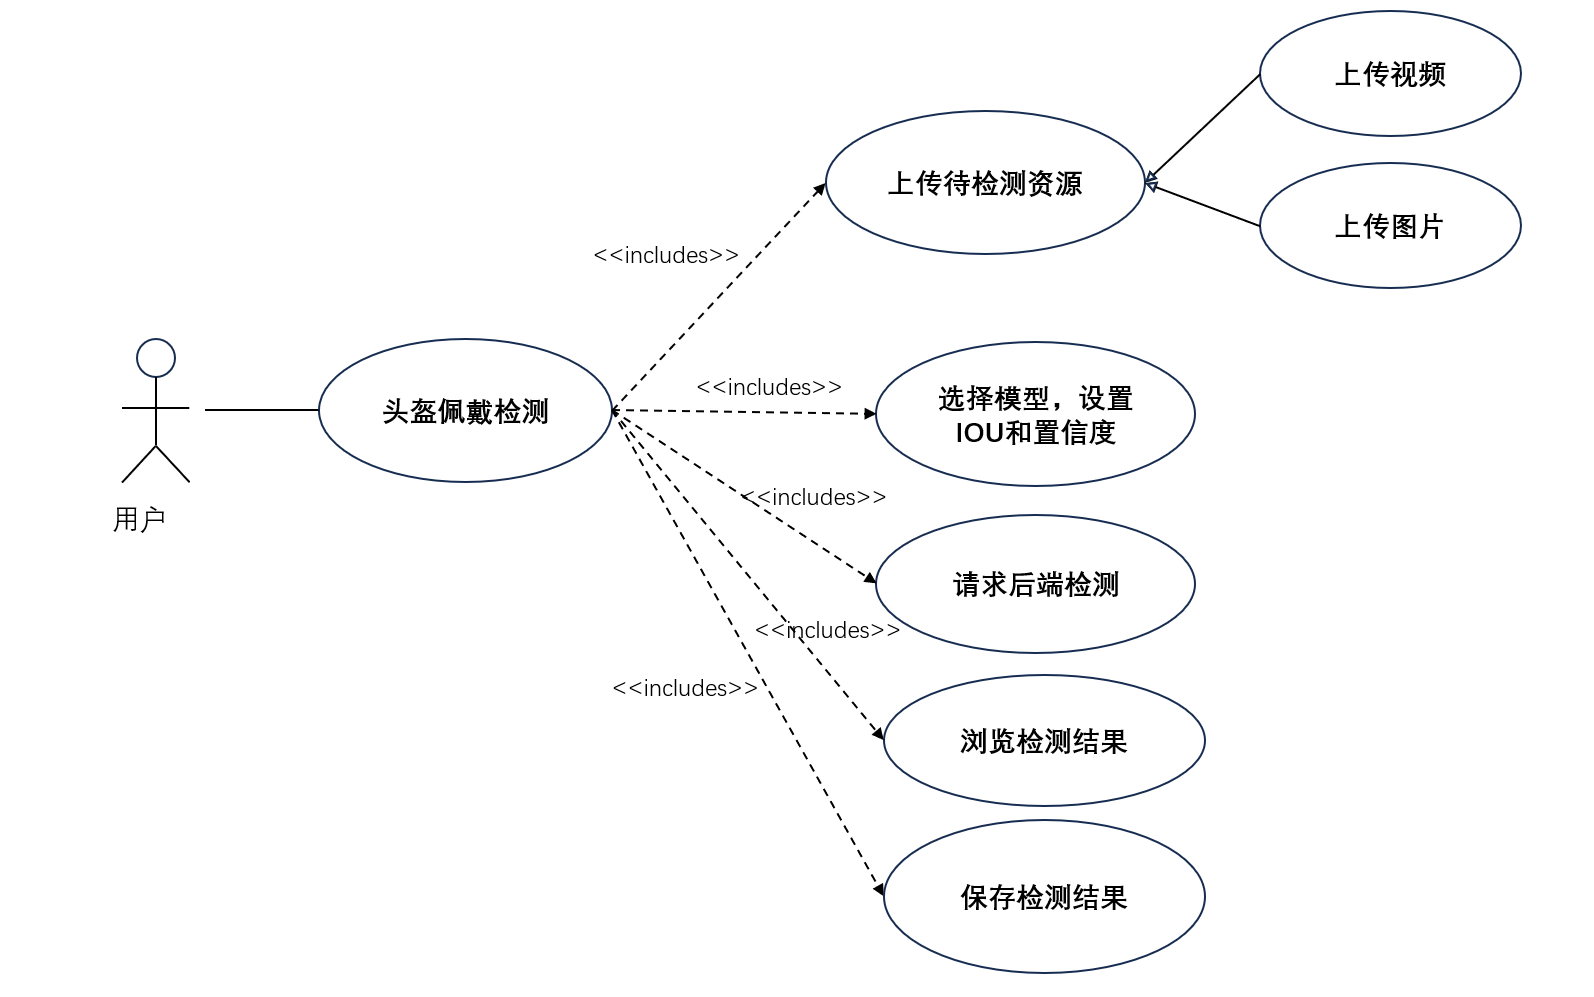
\includegraphics[width=0.9\textwidth]{figs/chap05/uml1.png}
    \caption{目标检测界面用例图}
    \label{fig:uml1}
\end{figure}

\ref{fig:seq1}展示了上述用例的交互顺序。用户需要先上传待检测资源,前端接收到资源后会展示在页面上。然后用户选择模型并调整参数,请求头盔佩戴检测功能。前端得到后端检测结果后,会将结果展示在页面上供用户浏览、保存。
\begin{figure}[!htb]
    \centering
    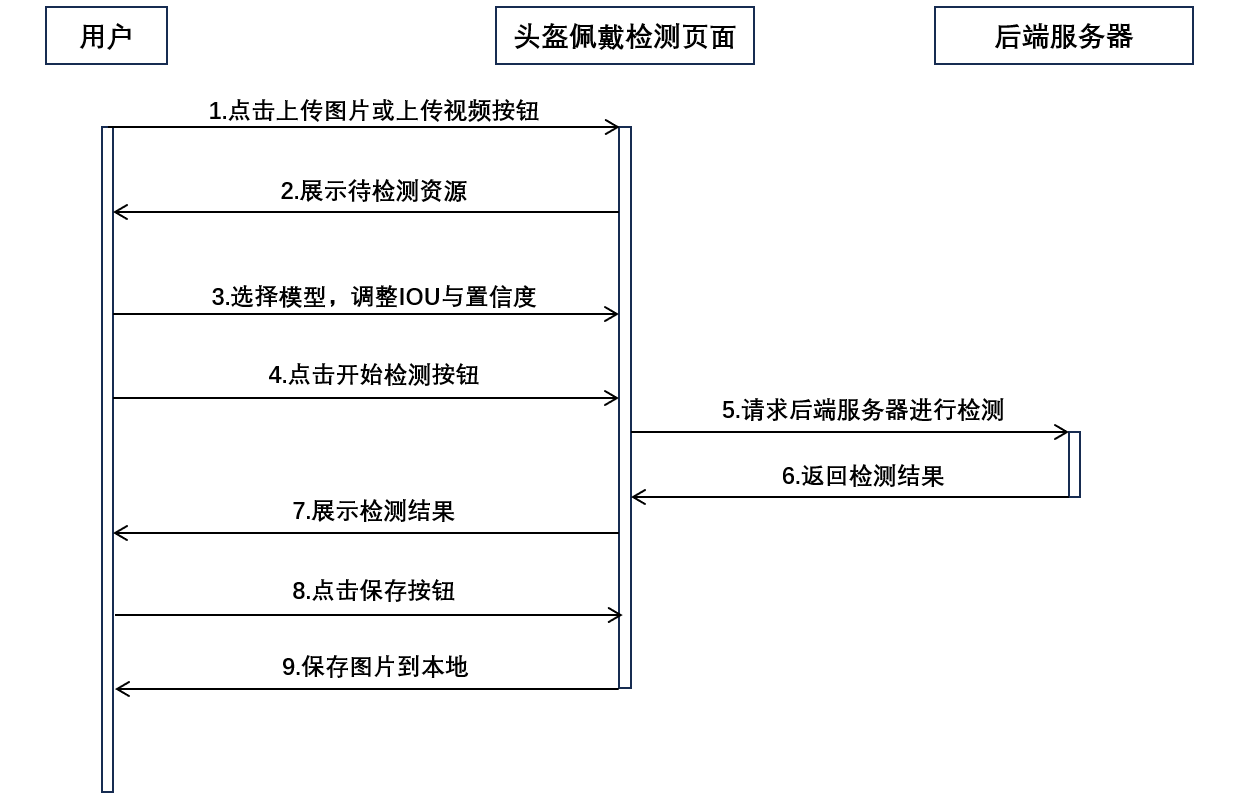
\includegraphics[width=0.95\textwidth]{figs/chap05/seq1.png}
    \caption{目标检测界面顺序图}
    \label{fig:seq1}
\end{figure}

目标检测界面的实现如\ref{fig:detAll}所示,核心是显示区、参数设置区、系统消息区和功能触发区。显示区用于浏览待检测资源和结果;功能触发区中,“上传图片”“上传视频” 按钮可上传待检测资源,“开始检测” 按钮请求后端检测,“保存结果” 按钮能将结果存至本地;参数设置区支持选择检测模型并设置IOU和置信度;系统消息区会展示用户操作情况。

\begin{figure}[H]
    \centering
    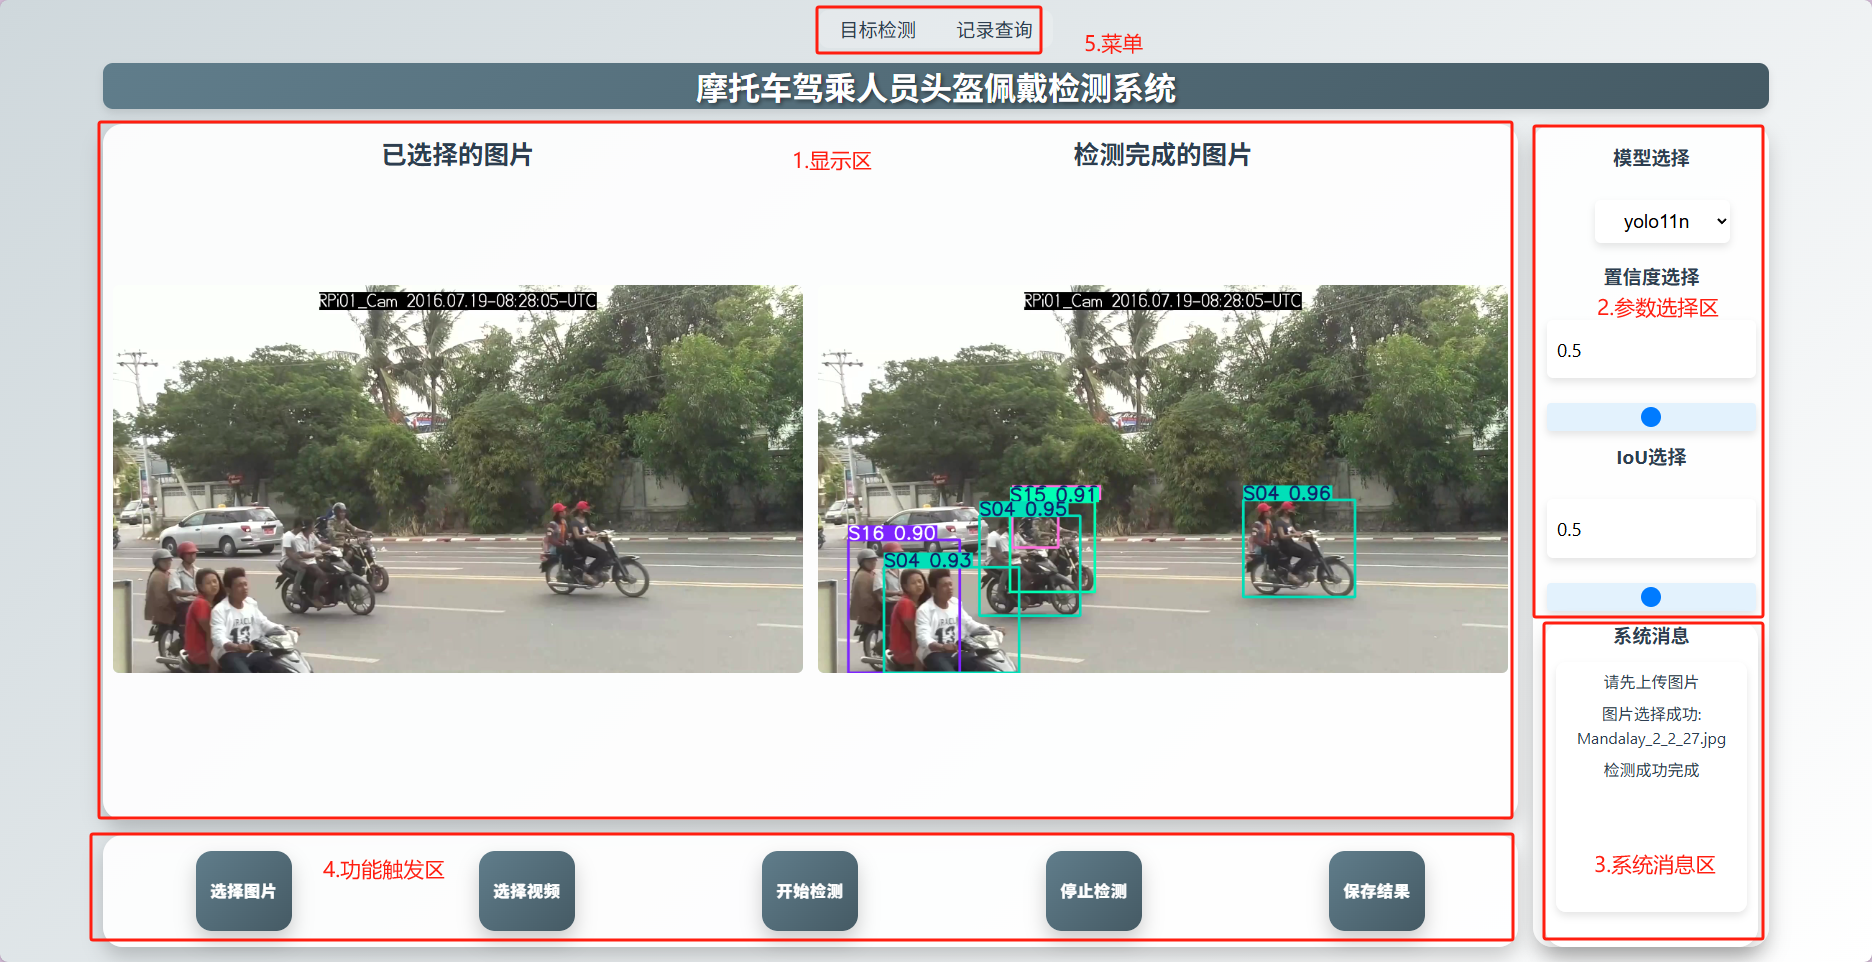
\includegraphics[width=0.95\textwidth]{figs/chap05/detAll.png}
    \caption{目标检测界面布局}
    \label{fig:detAll}
\end{figure}

% 显示区是页面中最大,最主要的区域,用于展示用户上传的原数据,以及检测结果。该区域被设置为flex布局,左右两边的图像在整个显示区是左右对称的,且大小相同。右侧参数设置区允许用户调整检测模型、Iou和置信度。右下方的系统消息区用来展示用户每一步的操作情况。下方的功能触发区给用户提供选择图片和视频、请求检测、终止当前检测以及保存检测结果的功能。最上方的菜单用于切换检测界面和查询界面。

% \subsubsection{功能测试}
% 首先对检测界面的参数设置区进行检测。对同一张图片,设置不同置信度参数。\ref{fig:conf1}和\ref{fig:conf2}分别展示了置信度设置为0.5和0.95时的检测情况。结果表明,当置信度从0.5调整为0.95后,模型漏检了三个目标。通过查看后台python脚本执行日志,用户能够选择不同的模型进行目标检测。

% \begin{figure}[!htb]
%     \centering
%     \begin{minipage}{0.45\textwidth} % 调整宽度以适应需求,两张图总宽度接近1
%         \centering
%         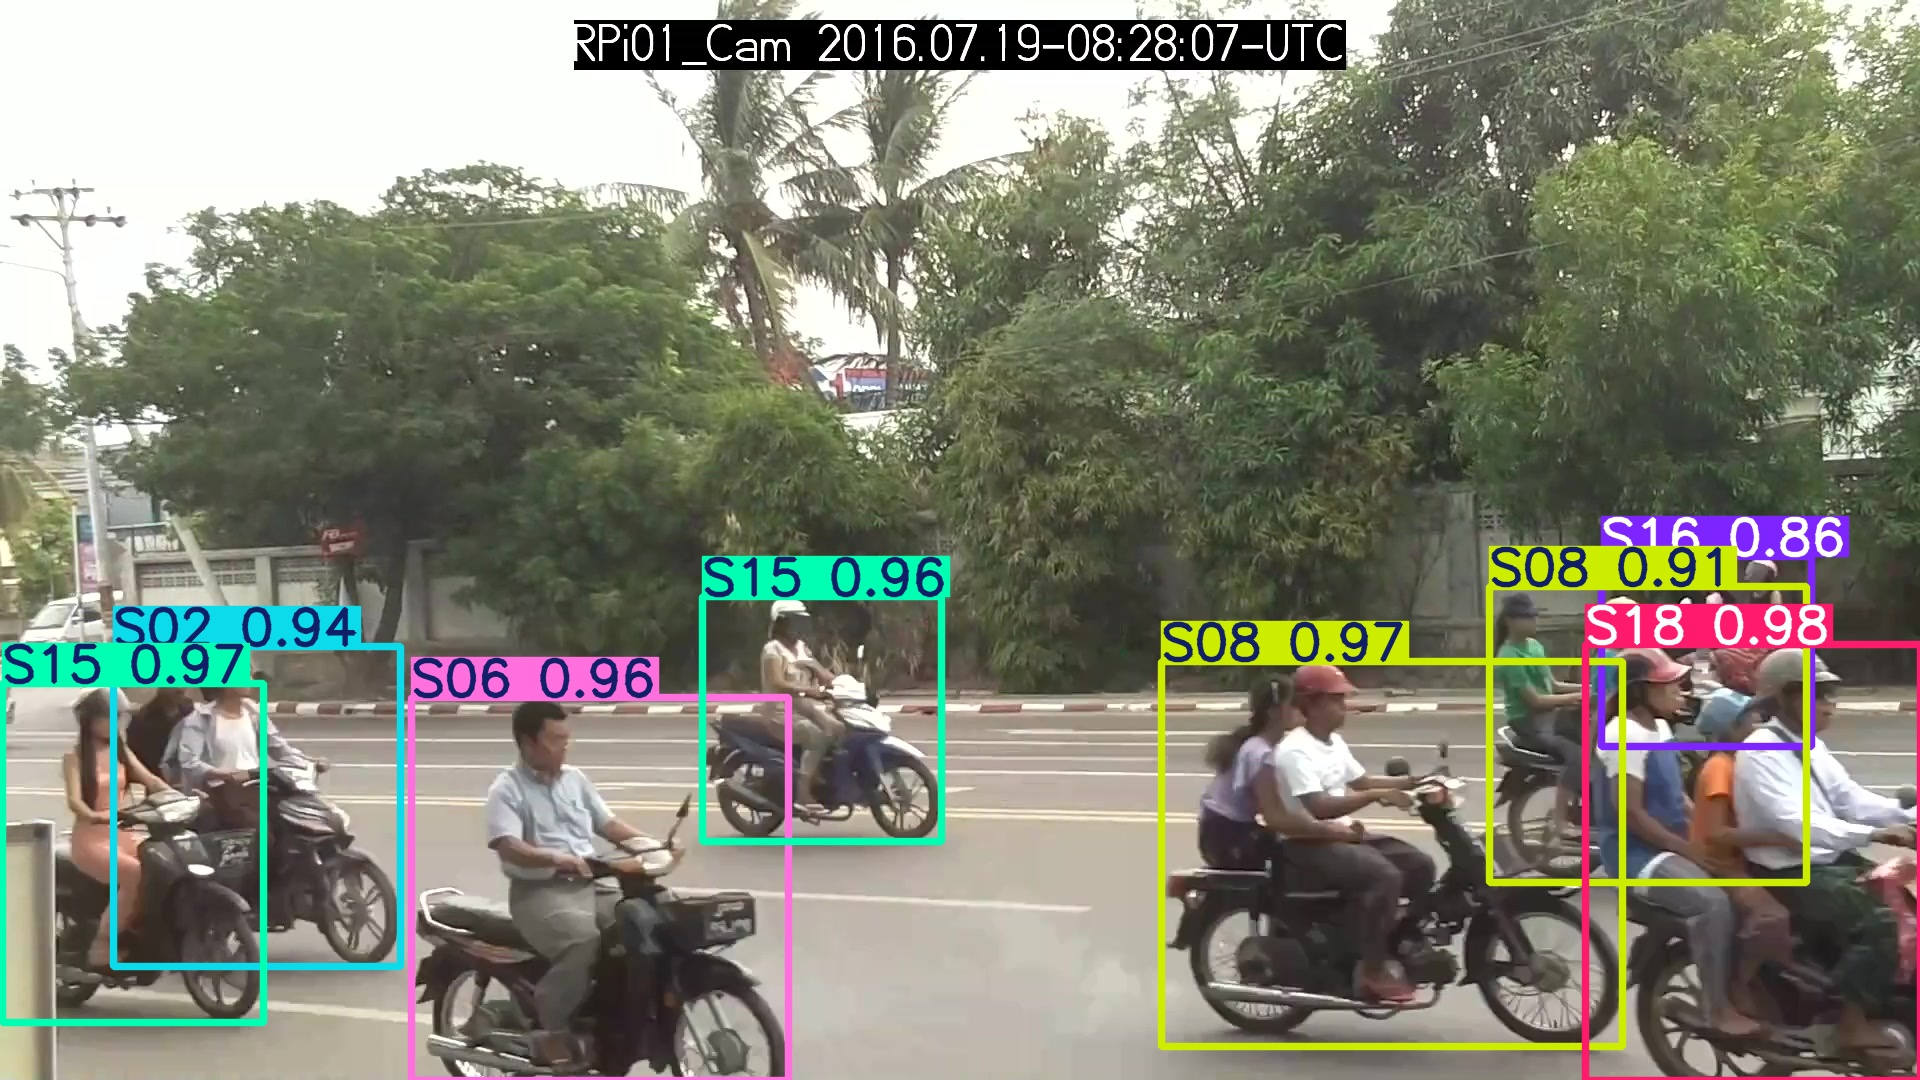
\includegraphics[width=\textwidth]{figs/chap05/conf1.jpg}
%         \caption{置信度0.5}
%         \label{fig:conf1}
%     \end{minipage}
%     \hfill % 使两张图片之间保持一定距离
%     \begin{minipage}{0.45\textwidth}
%         \centering
%         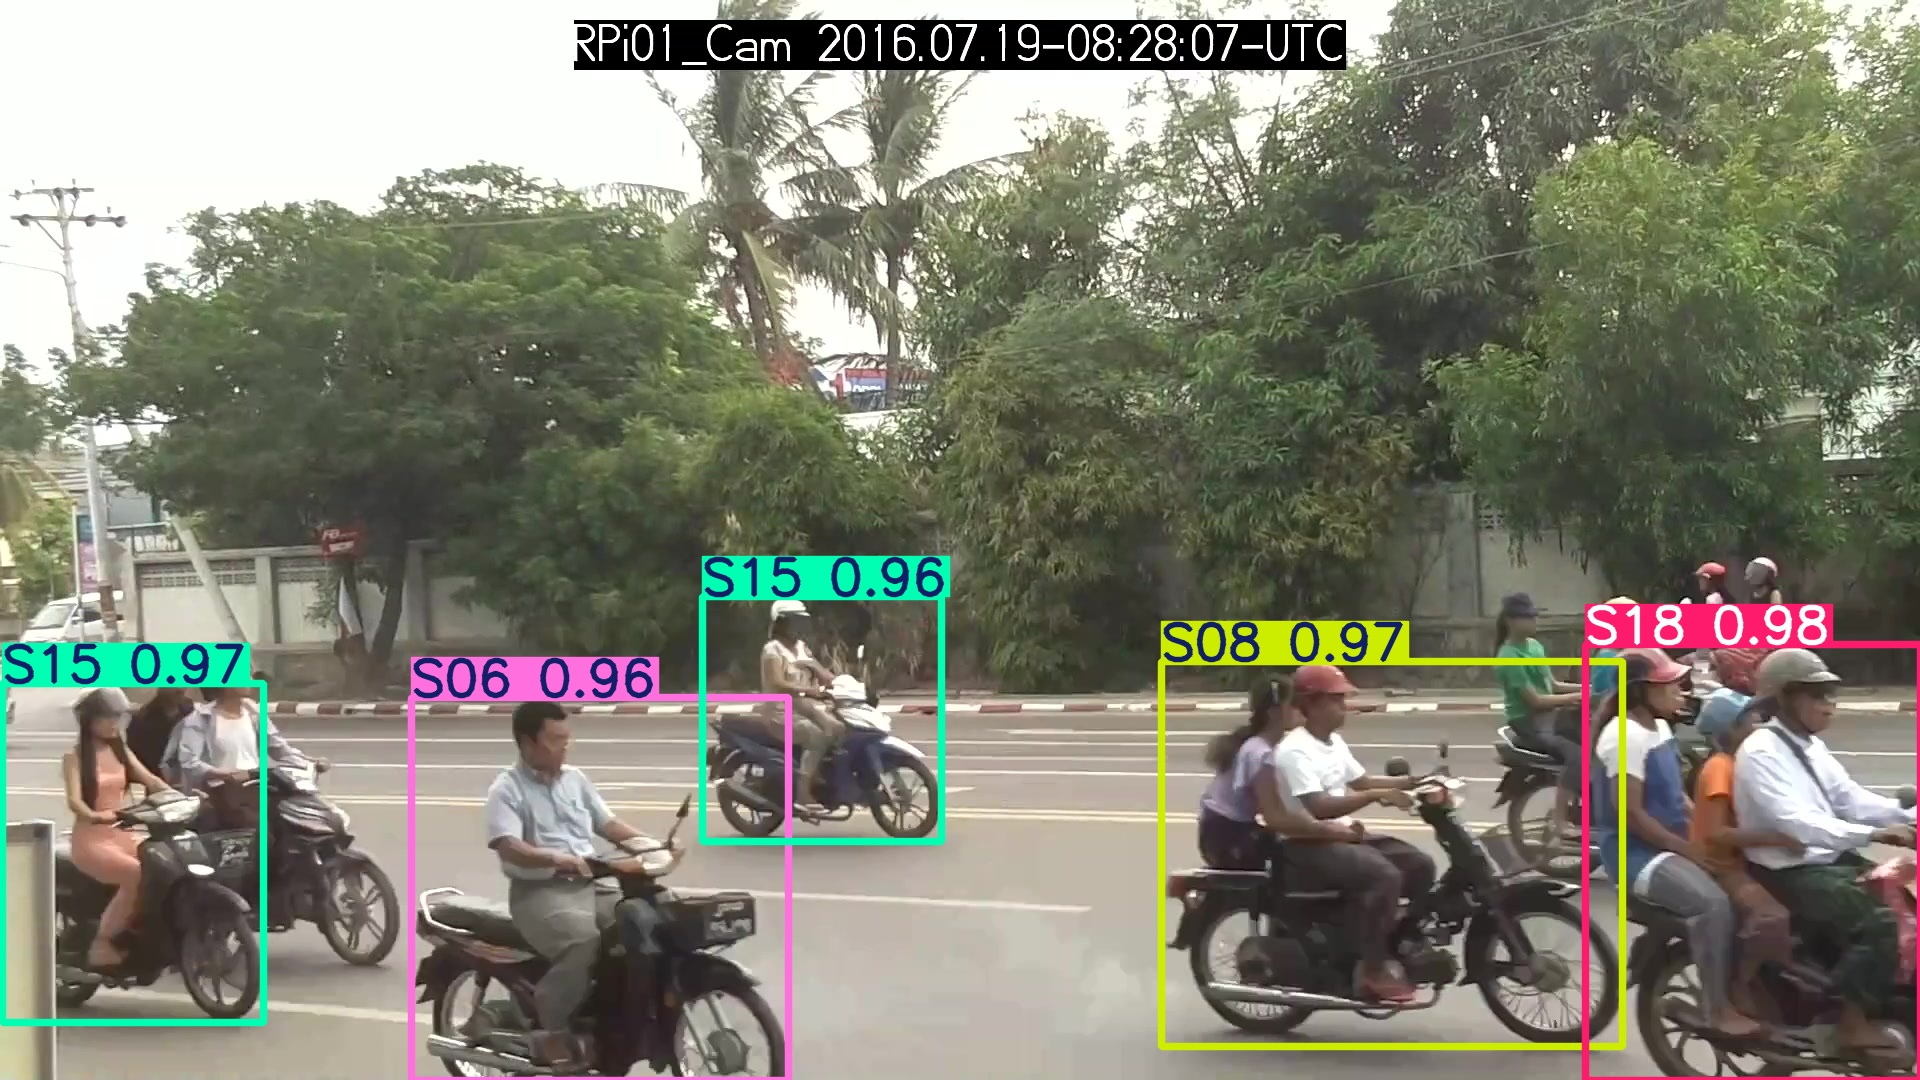
\includegraphics[width=\textwidth]{figs/chap05/conf2.jpg}
%         \caption{置信度0.95}
%         \label{fig:conf2}
%     \end{minipage}
%   \end{figure}

% 然后对下方的功能触发区进行测试。该系统除了图片之外,还支持用户上传视频进行检测。经测试,上传视频并进行检测的功能可以正常使用,效果如\ref{fig:video}所示。且用户点击保存结果后,会触发浏览器的下载功能,将检测结果保存到本地。在整个测试过程中,系统消息区可以将用户的操作结果正确展示出来。

% \begin{figure}[!htb]
%     \centering
%     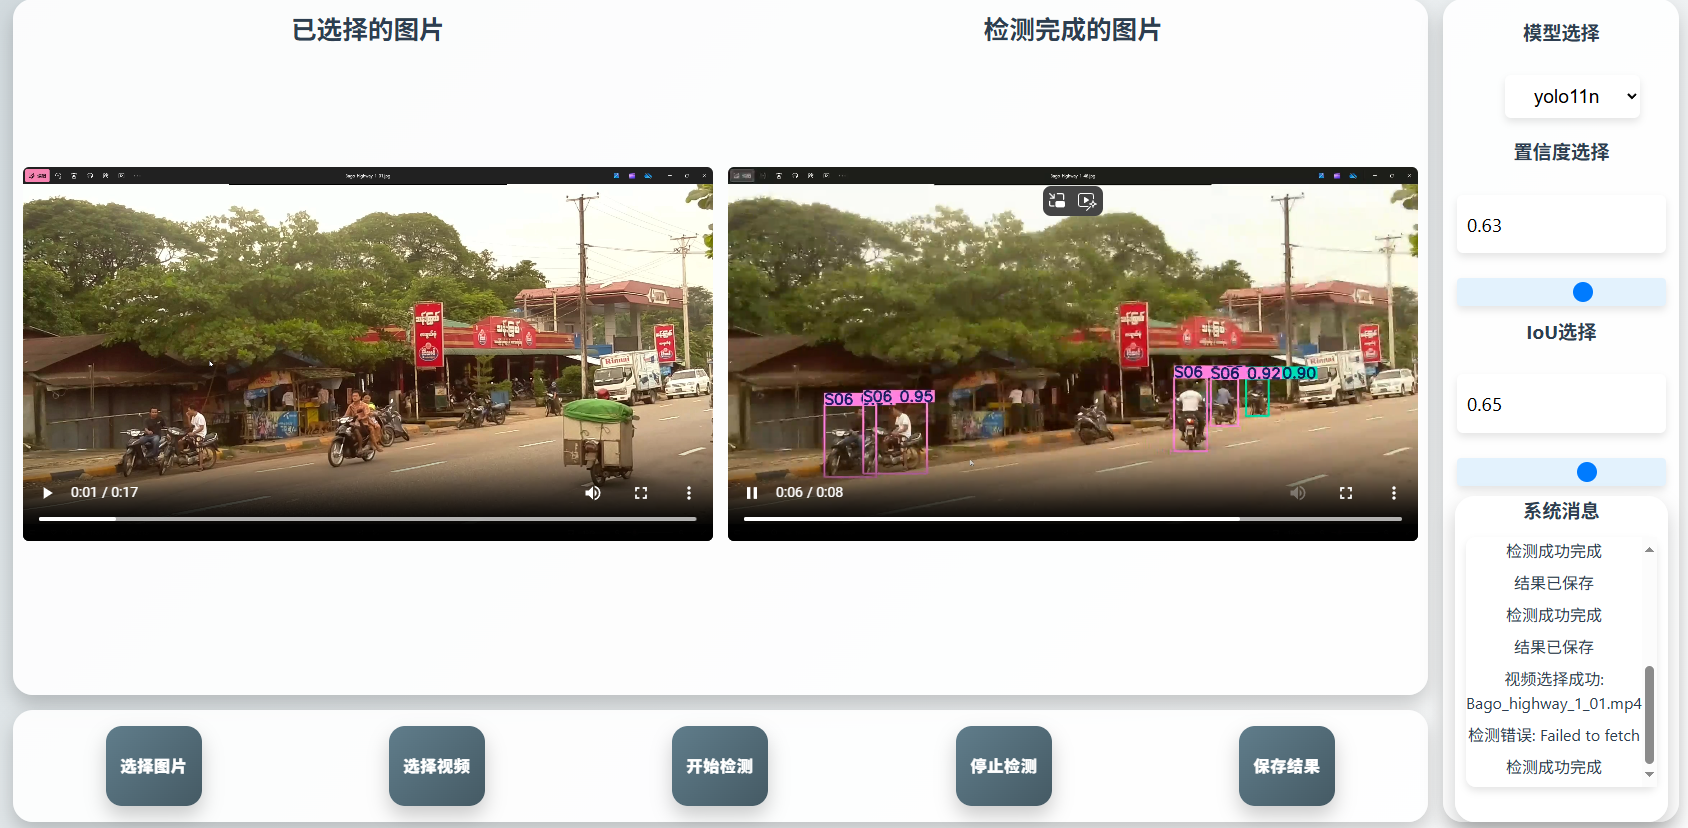
\includegraphics[width=0.9\textwidth]{figs/chap05/video.png}
%     \caption{视频检测测试}
%     \label{fig:video}
% \end{figure}

\subsection{记录查询界面}
% \subsubsection{界面布局}
记录查询界面用例设计如\ref{fig:uml2}。该页面以历史记录查询用例为核心。改用例包含设置查询过滤条件、请求后端查询和数据可视化三个子用例。设置查询过滤条件分为设置驾驶员、检测地点和检测时间三个子用例,允许用户对着三个字段设置过滤条件。通过请求查询用例发起查询请求。得到的查询结果会通过数据可视化用例通过图标的形式展示,提供了柱状图、折线图和饼图三种实现方式。

\begin{figure}[!htb]
    \centering
    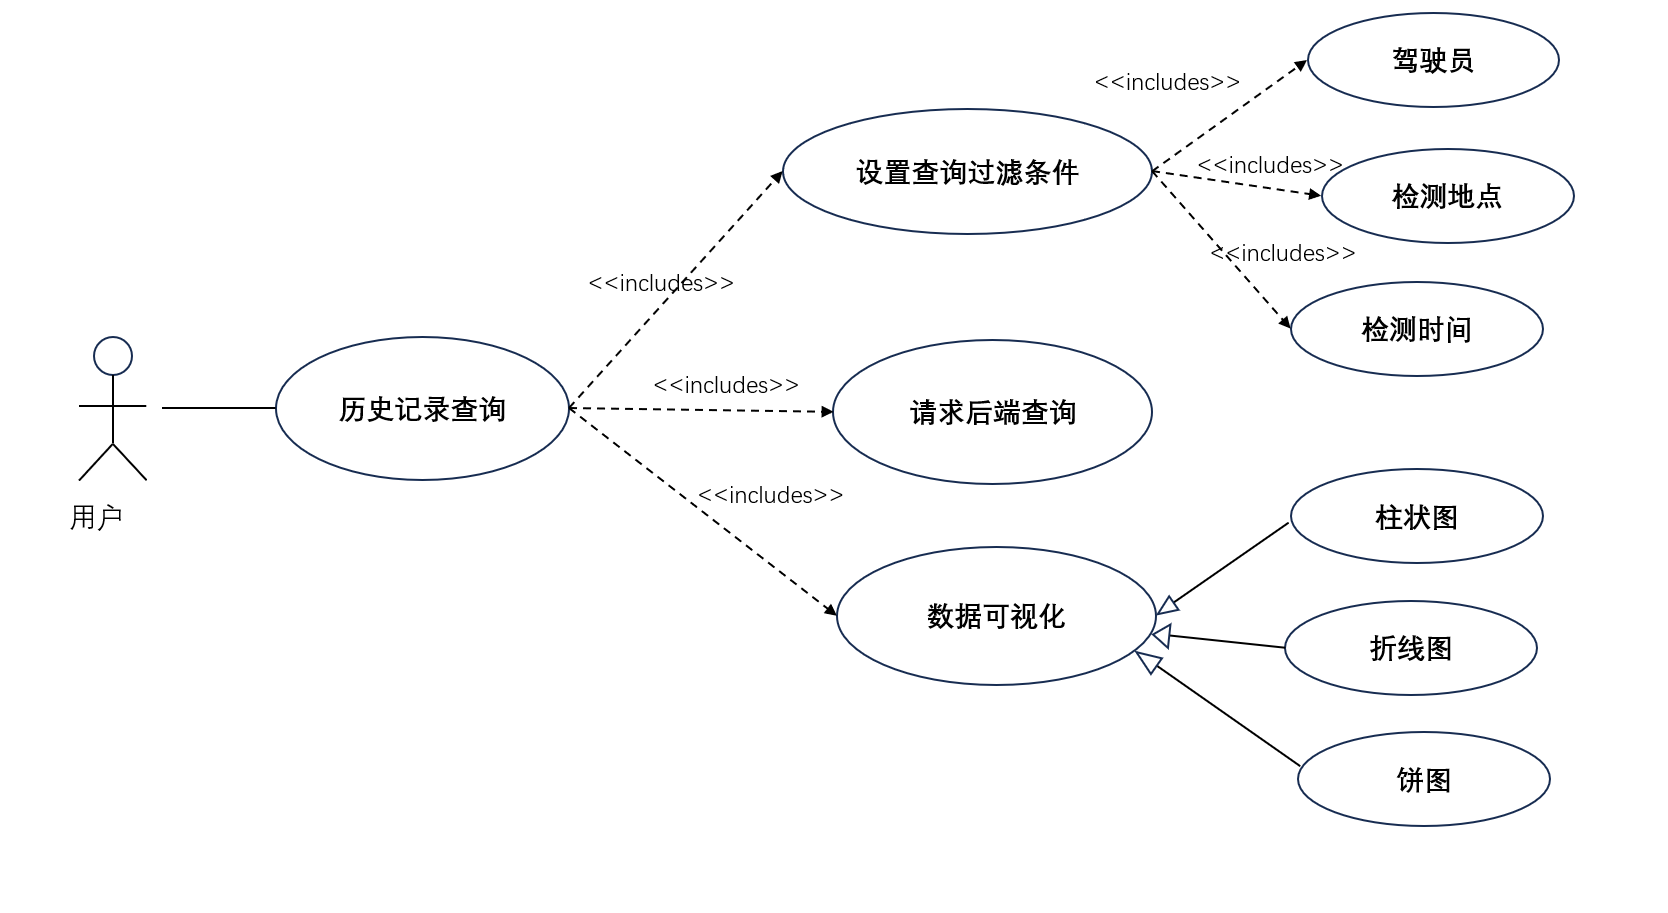
\includegraphics[width=0.95\textwidth]{figs/chap05/uml2.png}
    \caption{记录查询界面用例图}
    \label{fig:uml2}
\end{figure}

该页面的顺序图为\ref{fig:seq2}。用户需要先对驾驶员、检测地点和检测时间这三个字段设置查询过滤条件,不设置则认为不对该字段进行过滤,然后点击搜索按钮,前端页面会附带过滤条件向后端服务器发起查询请求。查询结果返回后,默认会展示柱状图类型的可视化图标,用户可以点击不同的图标类型选择不同的数据可视化方式。

\begin{figure}[!htb]
    \centering
    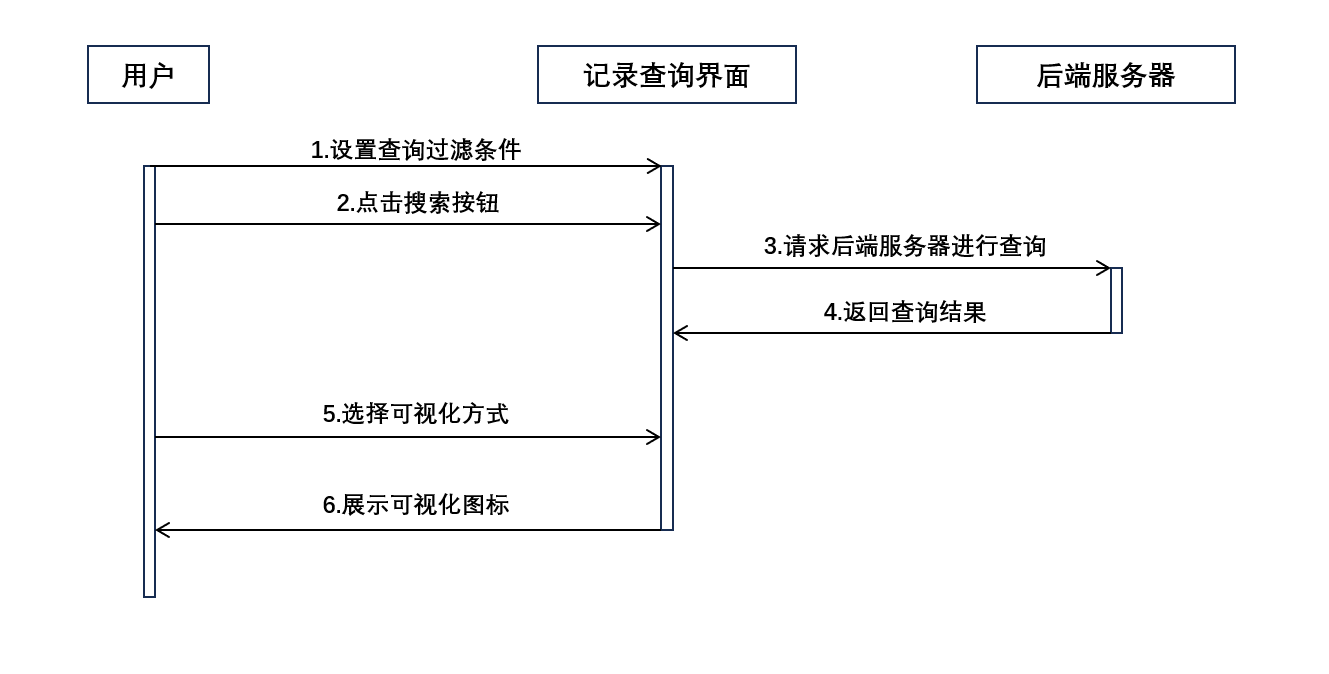
\includegraphics[width=0.95\textwidth]{figs/chap05/seq2.png}
    \caption{记录查询界面顺序图}
    \label{fig:seq2}
\end{figure}


记录查询界面的实现见\ref{fig:search}。用户通过记录查询区设置过滤条件并发起查询请求,查询结果会在数据可视化区以图标的形式展示,并允许用户选择不同的可视化方式。

\begin{figure}[!htb]
    \centering
    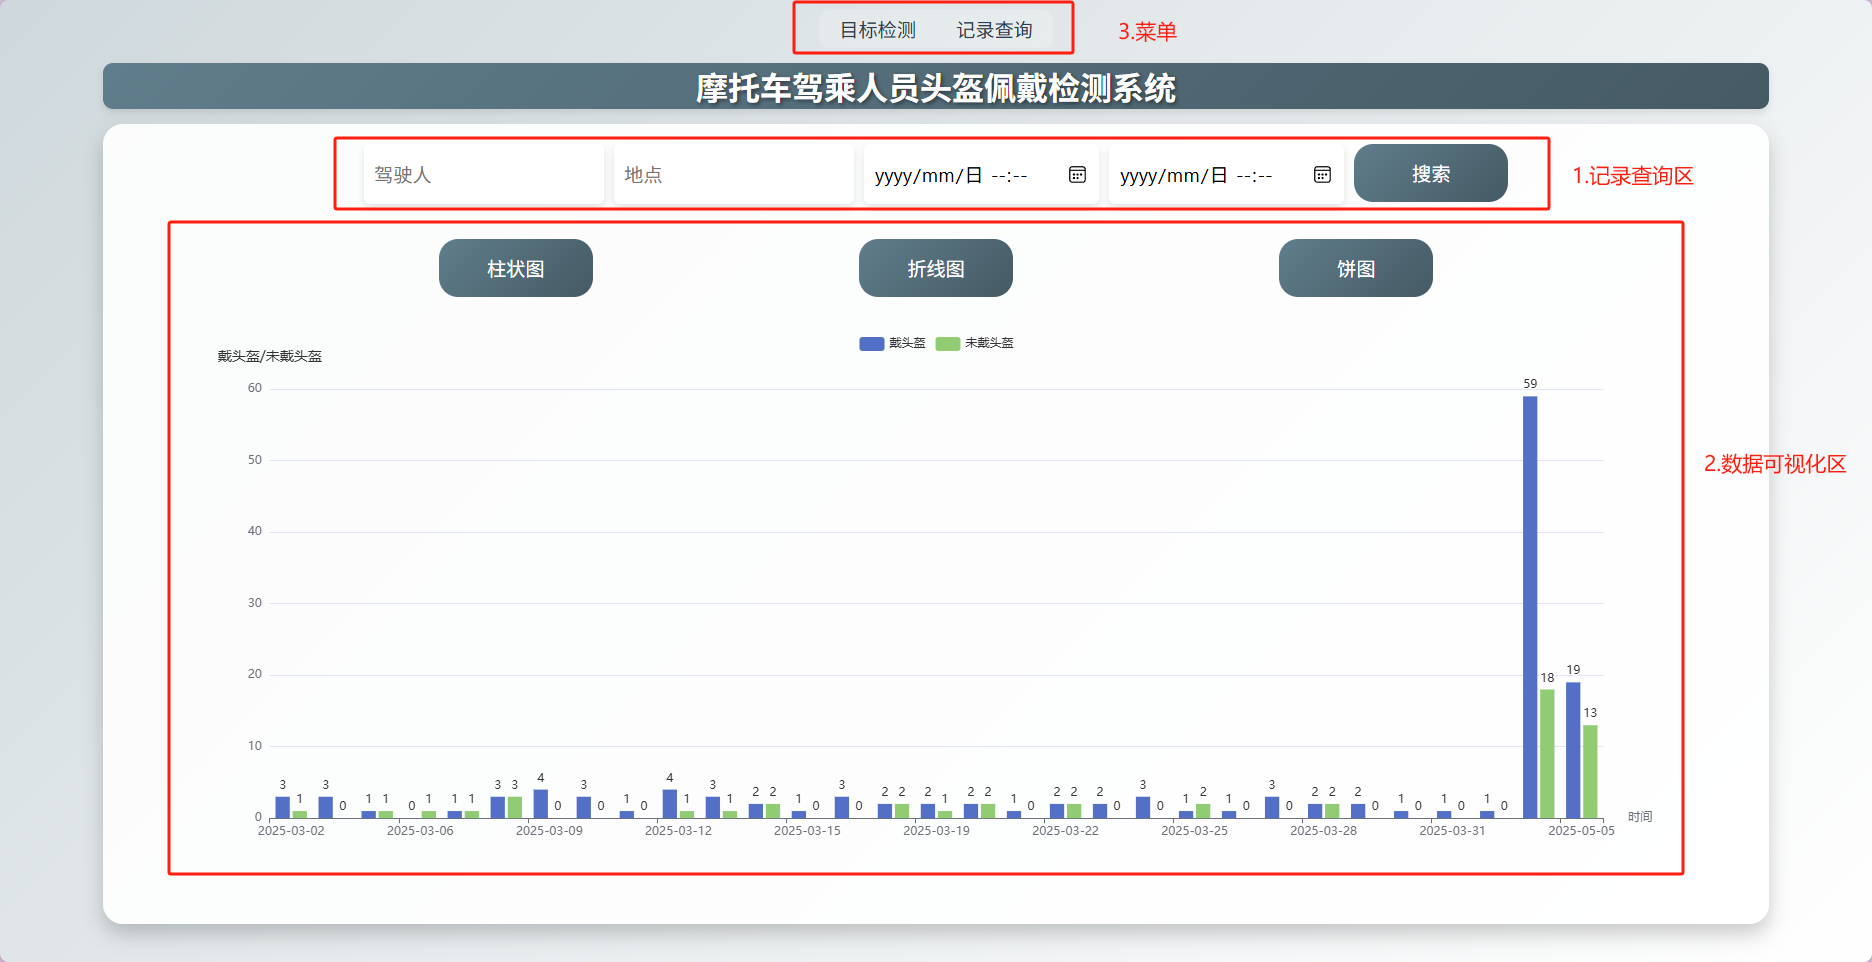
\includegraphics[width=0.95\textwidth]{figs/chap05/search.png}
    \caption{记录查询界面布局}
    \label{fig:search}
\end{figure}

% \subsubsection{功能测试}
% 对记录查询功能进行测试,设置为查询3月21日到5月5日的数据,可以通过下方的柱状图看出,过滤条件是生效的。切换不同的可视化图标,都可以展示正确结果。测试结果如\ref{fig:data1},\ref{fig:data2},\ref{fig:data3}。

% \begin{figure}[!htb]
%     \centering
%     \begin{minipage}{0.3\textwidth} % 调整宽度以适应需求,两张图总宽度接近1
%         \centering
%         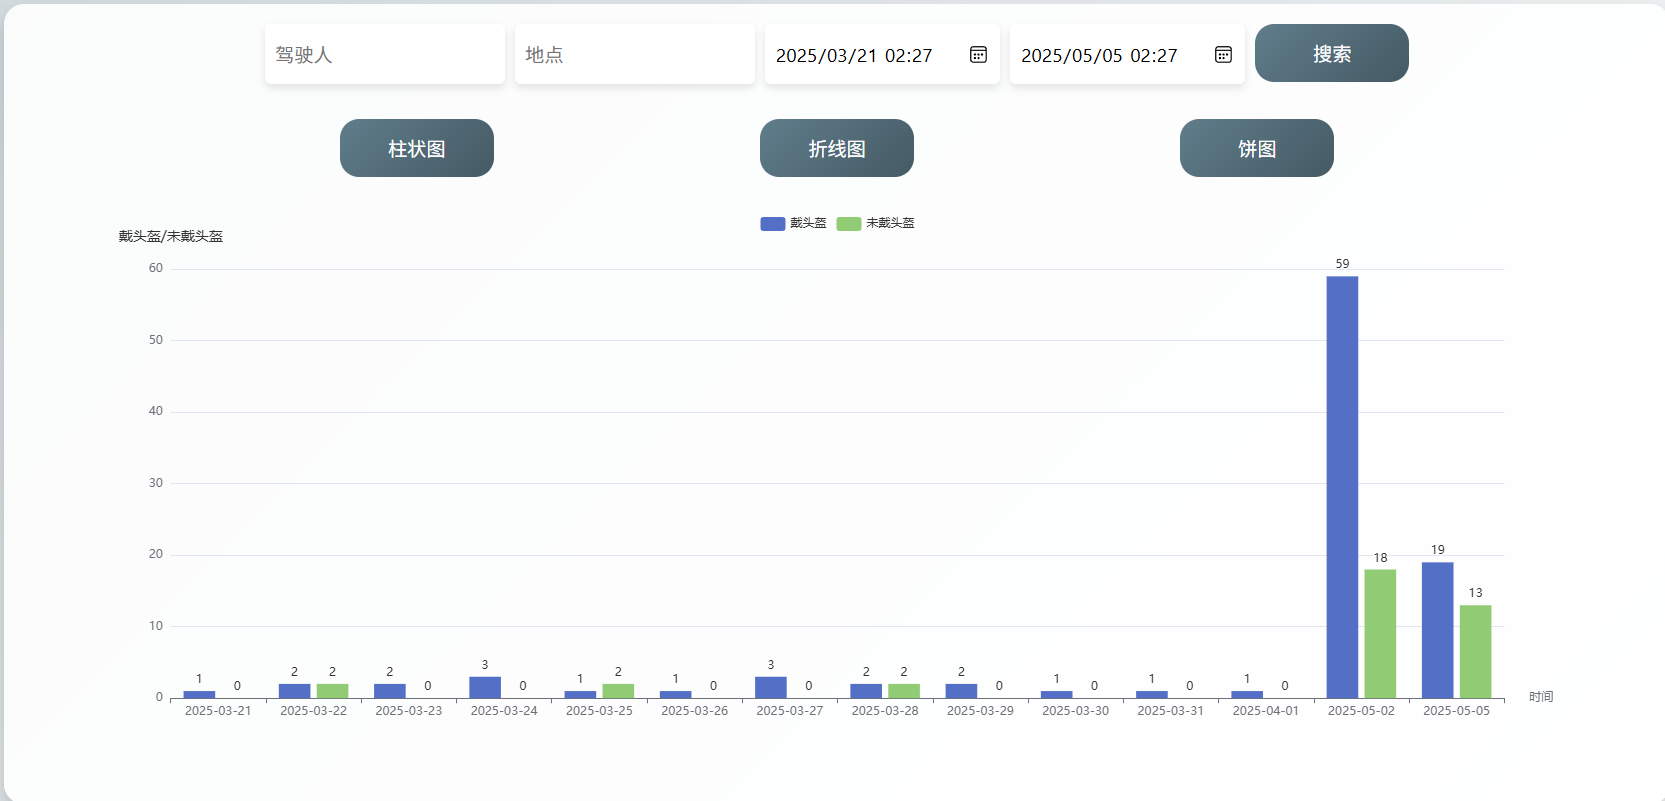
\includegraphics[width=\textwidth]{figs/chap05/data1.png}
%         \caption{柱状图}
%         \label{fig:data1}
%     \end{minipage}
%     \hfill % 使两张图片之间保持一定距离
%     \begin{minipage}{0.3\textwidth}
%         \centering
%         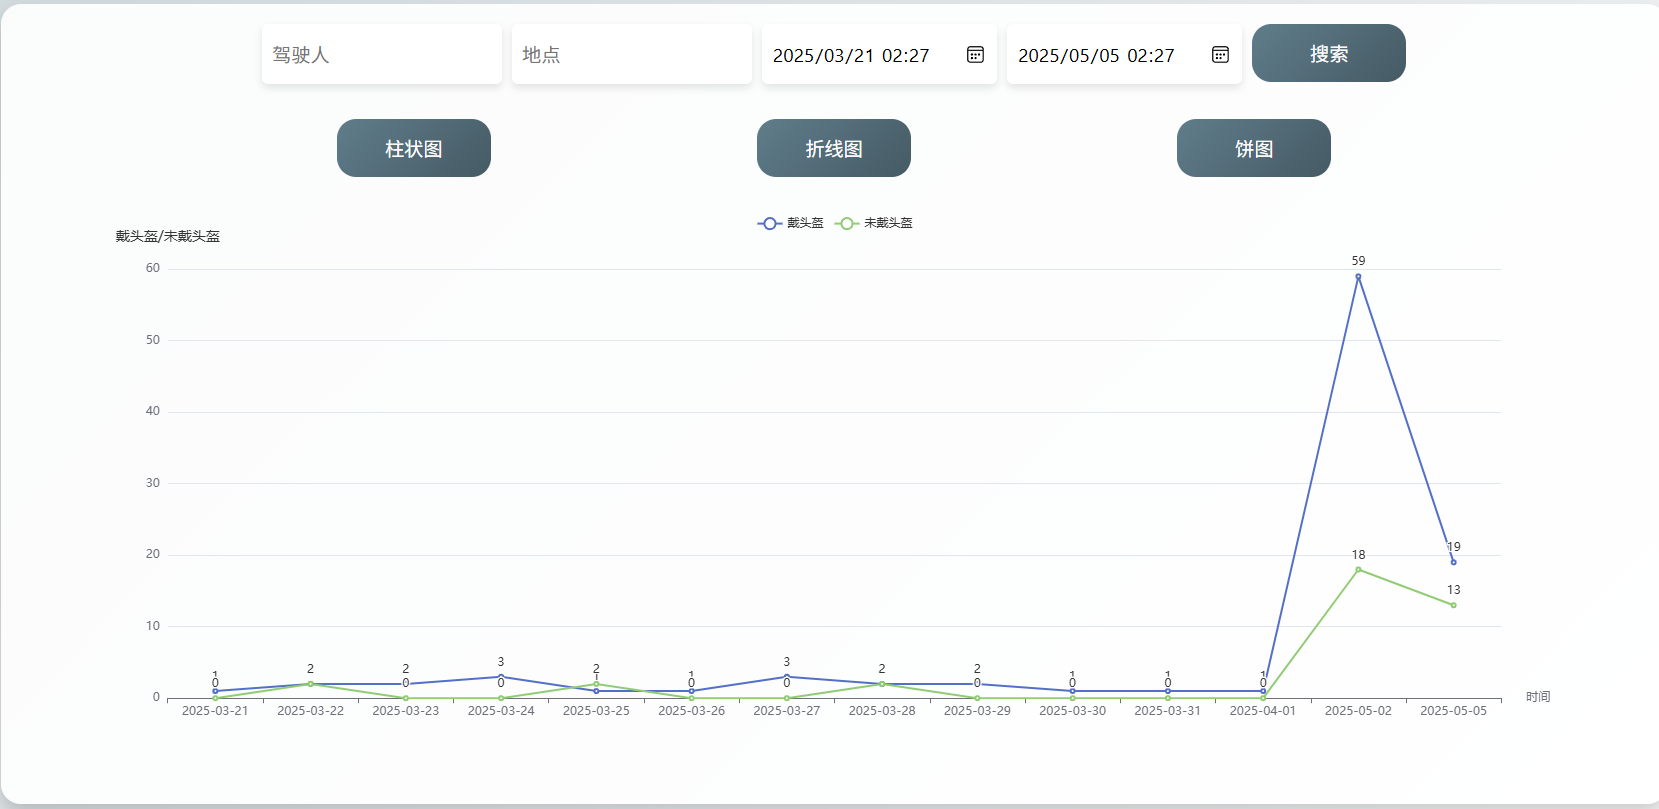
\includegraphics[width=\textwidth]{figs/chap05/data2.png}
%         \caption{折线图}
%         \label{fig:data2}
%     \end{minipage}    
%     \hfill % 使两张图片之间保持一定距离
%     \begin{minipage}{0.3\textwidth}
%         \centering
%         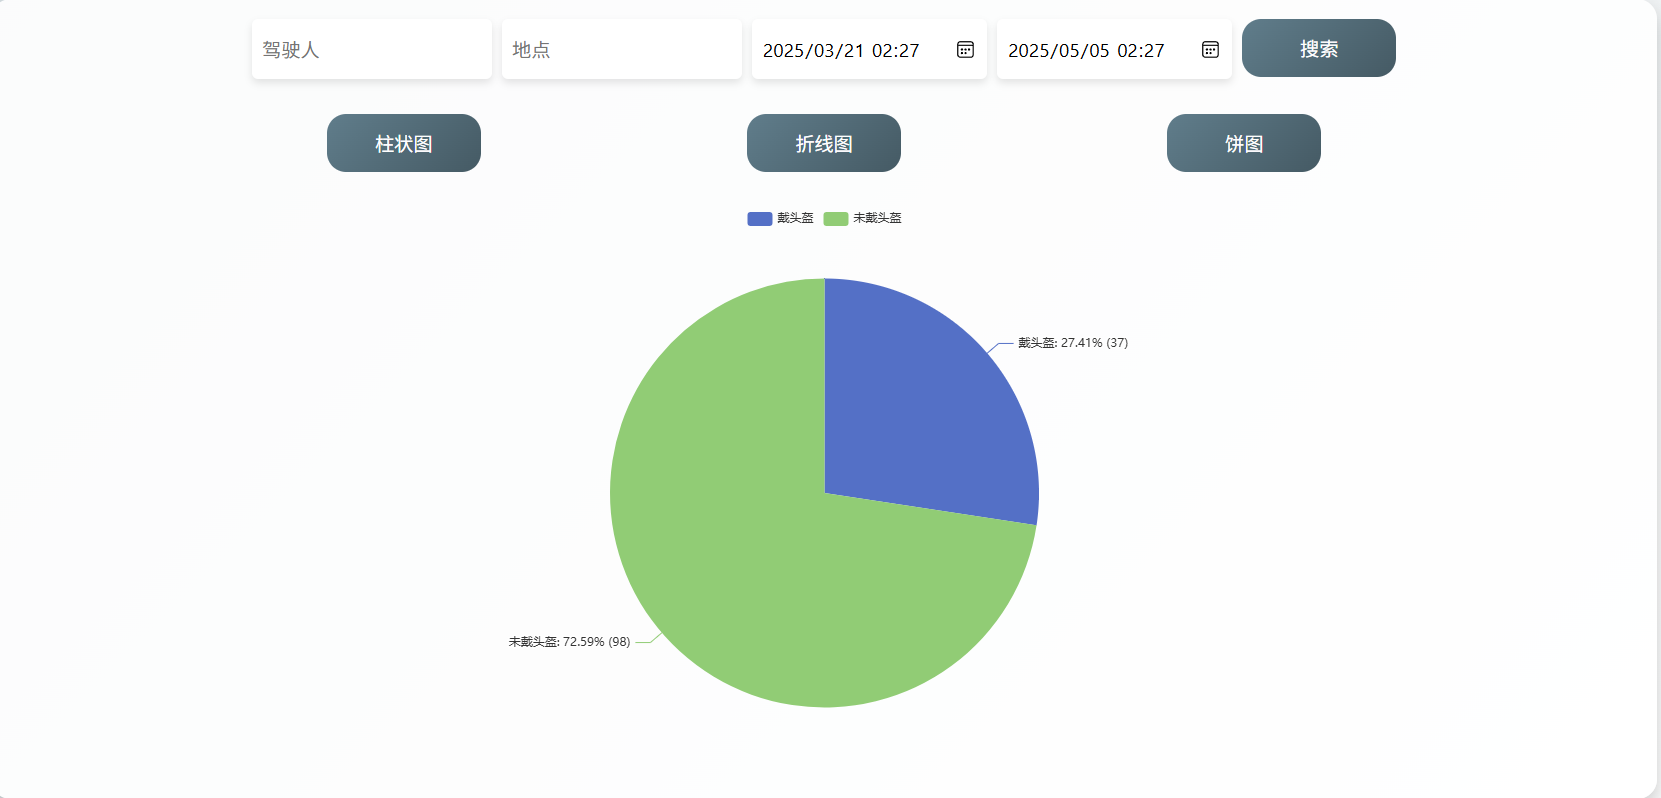
\includegraphics[width=\textwidth]{figs/chap05/data3.png}
%         \caption{饼图}
%         \label{fig:data3}
%     \end{minipage}
%   \end{figure}

\section{后端模块设计与实现}
后端模块在框架上选用SpringBoot进行开发,在架构上选择MVC三层架构。该系统主要分为两个模块:检测模块和搜索模块,负责实现前端页面提供的两大功能。

\subsection{库表结构}
该系统使用的库表结构如\ref{tab:datatable}所示。该表共有五个字段,除主键id外,记录了驾驶员信息、头盔佩戴情况、检测地区和检测时间。头盔佩戴情况在库表里面是以整型的方式记录的,节省空间且信息更加简洁,后端会对label和该字段的整型值做转换。由于在查询过程中,经常会对驾驶员信息和头盔佩戴情况这两个字段过滤,所以在设计的时候对这两个字段都创建了索引。

\begin{table}[htbp]
    \centering
    \caption{数据库表字段设计} % 表格标题,可根据实际情况修改
    \label{tab:datatable}
    \begin{tabular}{lccc} % l 表示左对齐,c 表示居中对齐,这里根据列数和对齐需求设置
        \toprule % 顶线
        字段 & 数据类型 & 说明 & 索引 \\
        \midrule % 中线
        id & int & 主键id & 主键索引 \\
        driver & varchar & 驾驶员 & 普通索引\\
        detect\_location & varchar & 检测地区 & 普通索引 \\
        helmet & int & 头盔佩戴情况 & 无 \\
        detect\_time & datetime & 检测时间 & 无 \\
        \bottomrule % 底线
    \end{tabular}
\end{table}

\subsection{检测模块}

后端检测模块的用例设计如\ref{fig:uml3}。该模块的核心用例是检测头盔佩戴,其包含保存待测资源、检测头盔佩戴情况、检测驾驶员id和返回结果四个子用例。保存待测资源会将用户上传的图片或视频保存到本地磁盘;检测头盔佩戴用例将调用模型对上述资源进行预测;检测驾驶员id包含两个子用例,首先通过驾驶员id识别模型进行身份判定,随后将模型输出的检测结果持久化存储至数据库,最终封装结果数据返回给前端。
\begin{figure}[!htb]
    \centering
    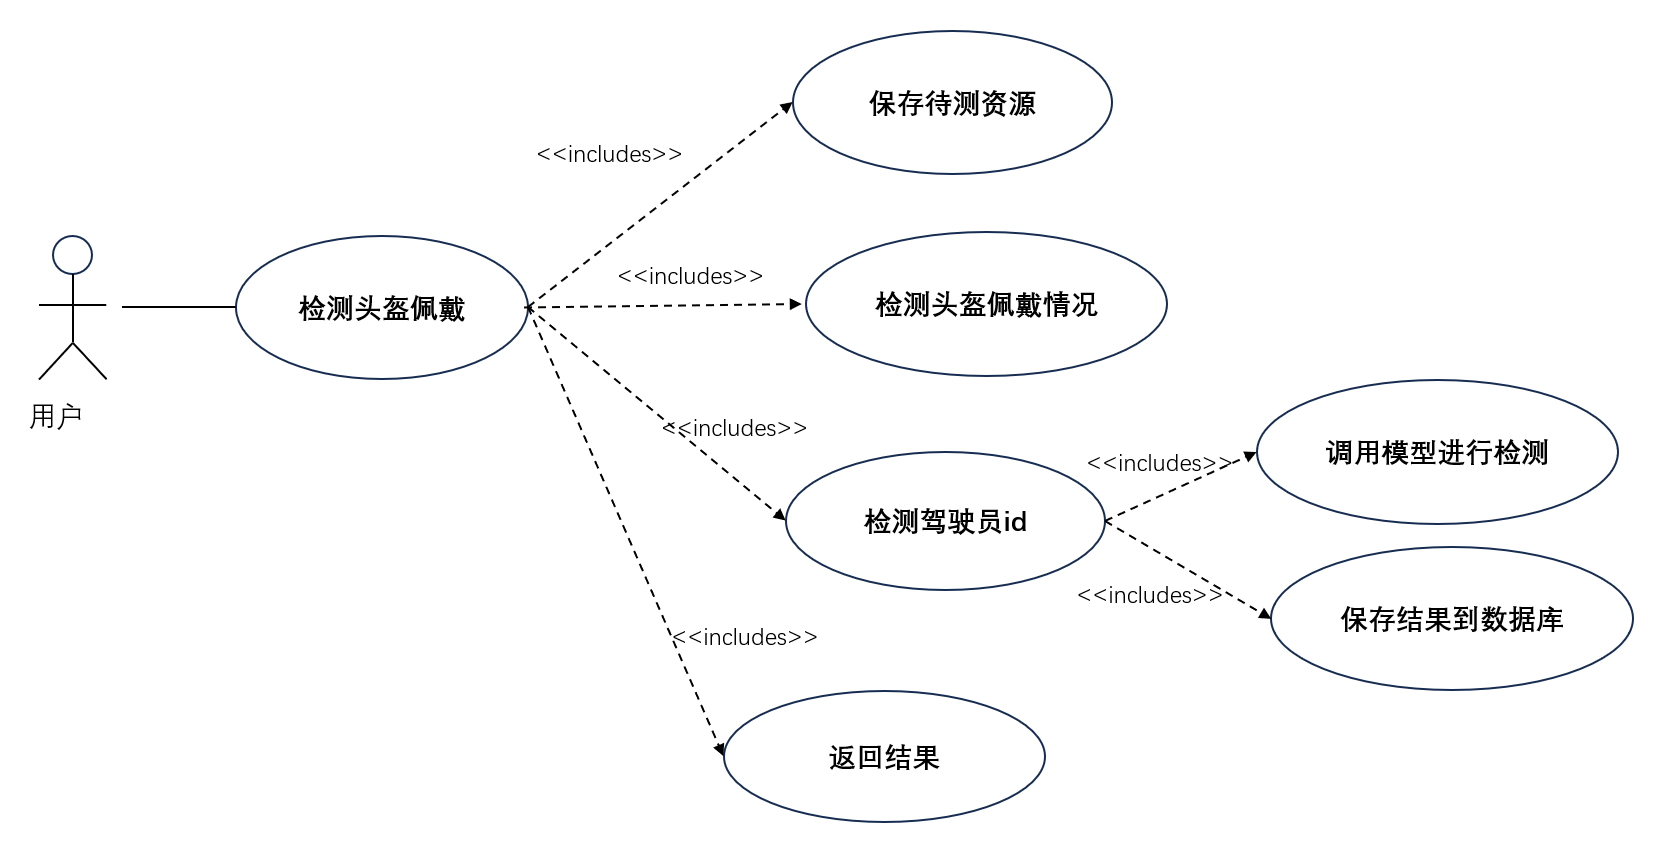
\includegraphics[width=0.95\textwidth]{figs/chap05/uml3.png}
    \caption{后端检测模块用例图}
    \label{fig:uml3}
\end{figure}

该模块执行顺序图如\ref{fig:seq3}。首先前端页面会上传待测资源到后端,后端将资源保存到本地磁盘,然后调用模型检测头盔佩戴情况,将检测结果保存到本地磁盘,再调用第二个模型检测驾驶员id,将包含头盔佩戴情况、驾驶员以及检测时间等完整信息保存到数据库,最后封装结果返回给前端用户。

\begin{figure}[!htb]
    \centering
    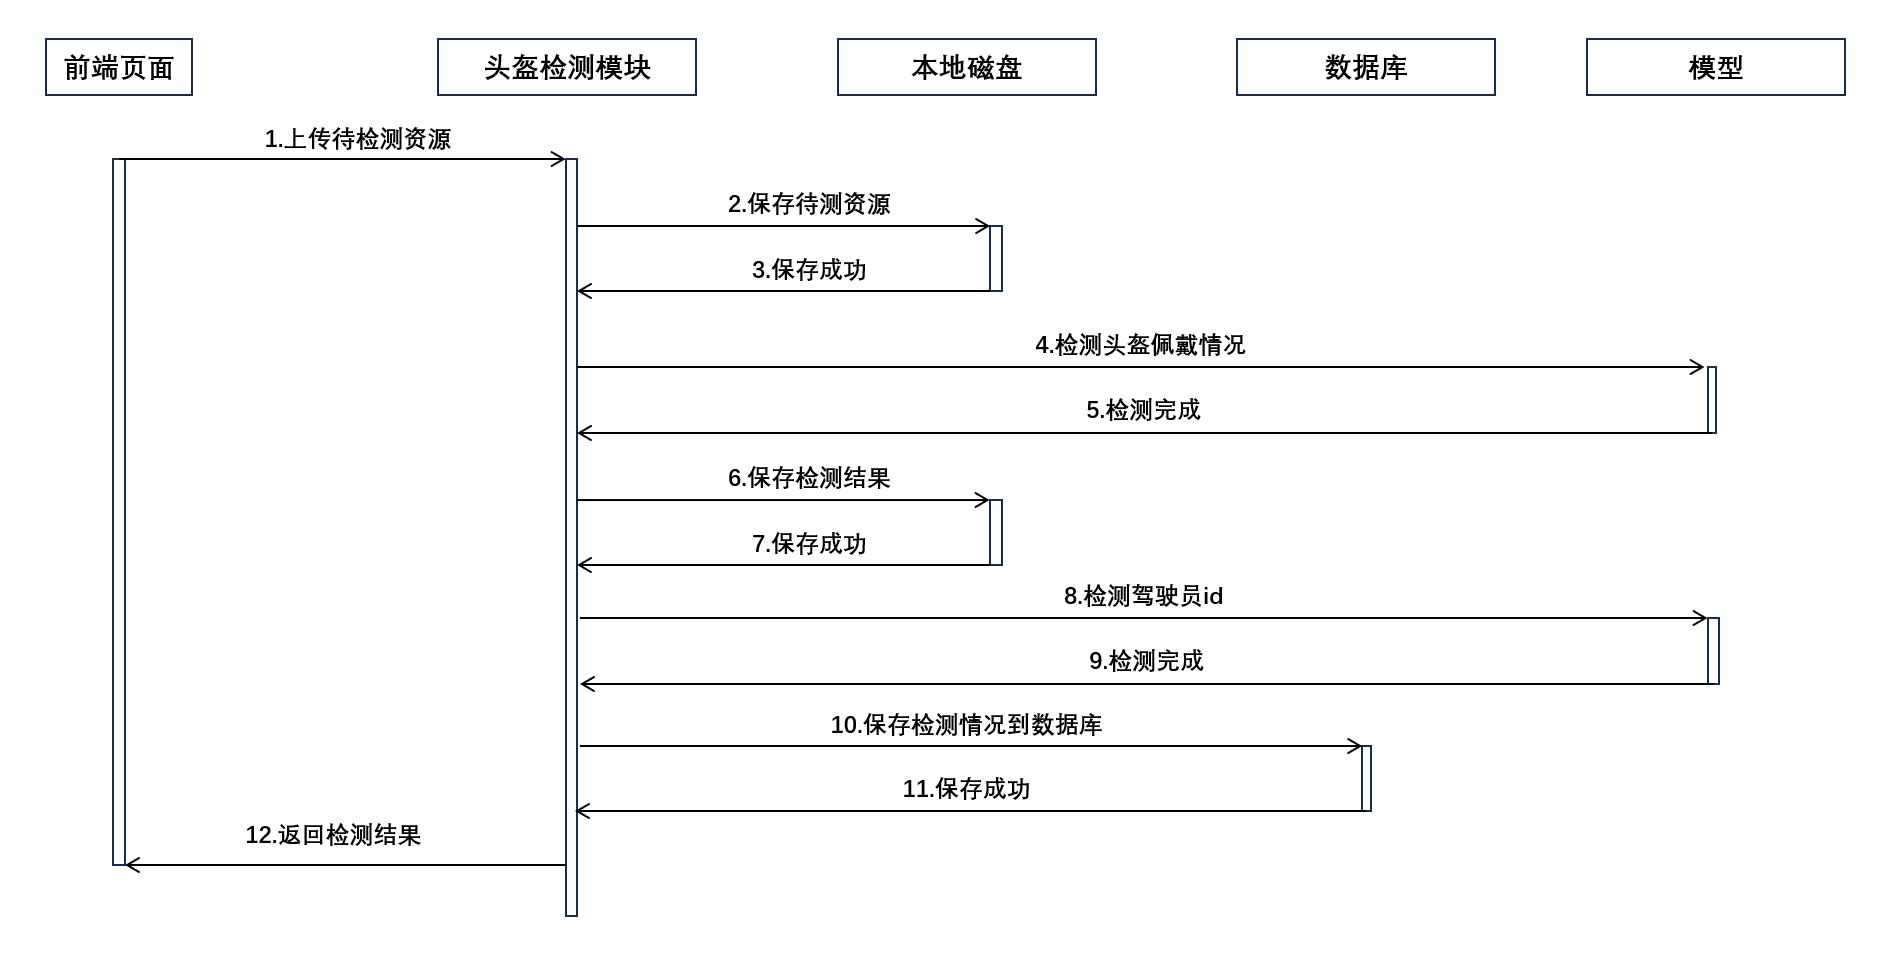
\includegraphics[width=0.95\textwidth]{figs/chap05/seq3.png}
    \caption{后端检测模块顺序图}
    \label{fig:seq3}
\end{figure}

该模块类图如\ref{fig:class1}所示,主要由DetectServiceImpl、ImageDTO和Detection三个类构成。ImageDTO类存储了用户输入的待检测资源和自定义检测模型、IOU和置信度四个参数。DetectServiceImpl的公共方法detect接收ImageDTO参数,其余私有方法分别负责保存待测资源、检测头盔佩戴、检测驾驶员id、保存检测结果和构建返回结果,如果当前是视频资源,还会将格式从avi转换为mp4。DetectServiceImpl关联的Detection类作为saveDetectResult()方法的输入参数,负责保存检测结果,包括主键id、驾驶员、头盔佩戴情况、检测地点和检测时间五个属性。

\begin{figure}[!htb]
    \centering
    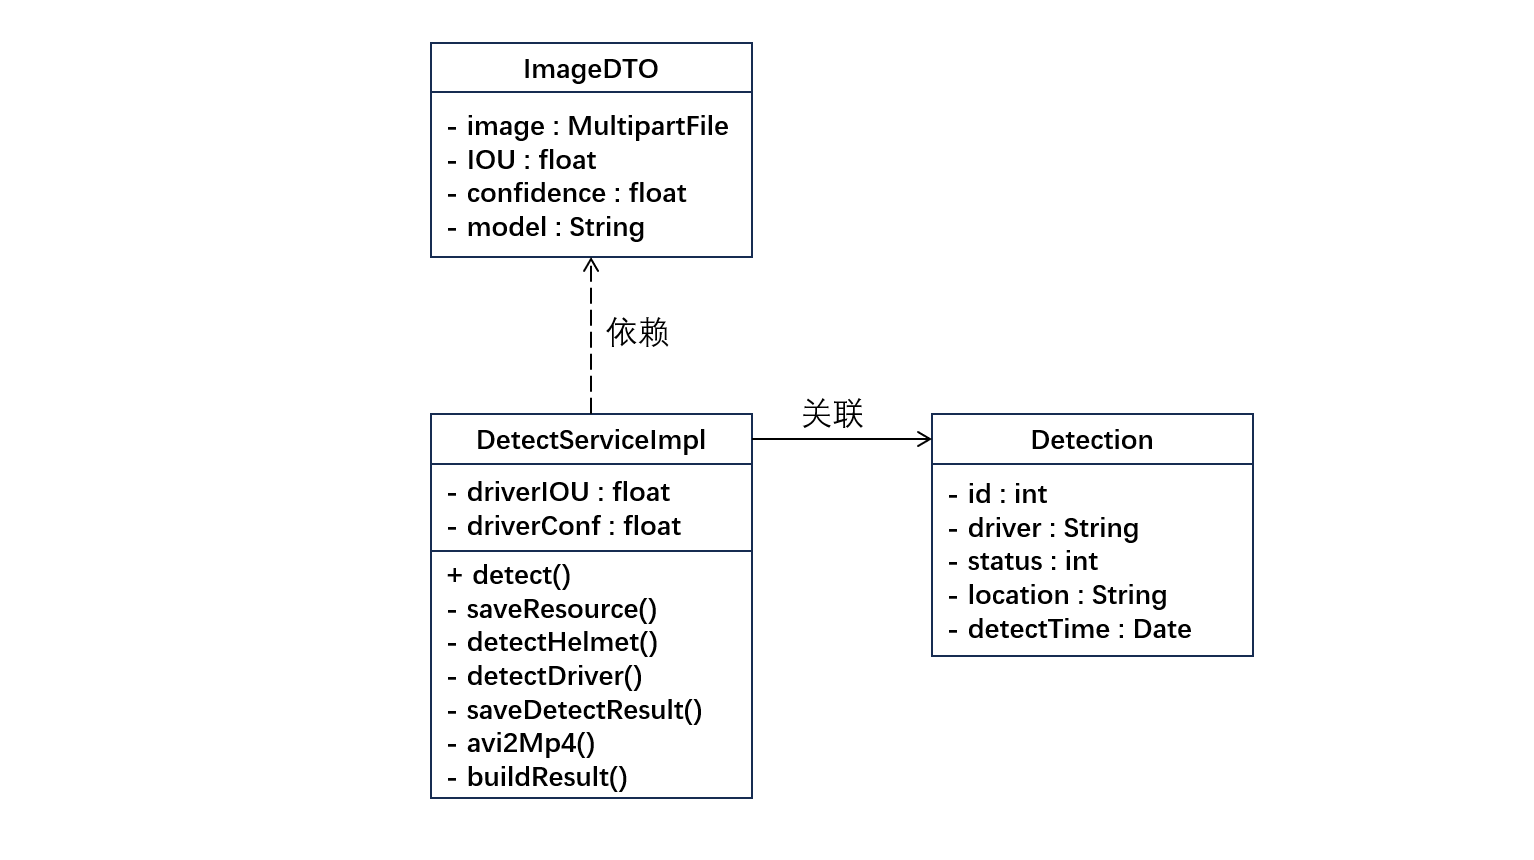
\includegraphics[width=0.9\textwidth]{figs/chap05/class1.png}
    \caption{后端检测模块类图}
    \label{fig:class1}
\end{figure}

\subsection{搜索模块}

后端搜索模块的用例图如\ref{fig:uml4}。该模块的核心用例是查询历史记录。其包含查询数据库、构建可视化图表数据格式和返回结果三个子用例。查询数据库包含获取过滤条件和执行sql语句两个子用例,这一步可以将用户需要的数据从数据库查询出来。构建柱状图、折线图和饼图三种图表特定的数据格式,支持前端进行数据可视化。最后返回查询结果。

\begin{figure}[!htb]
    \centering
    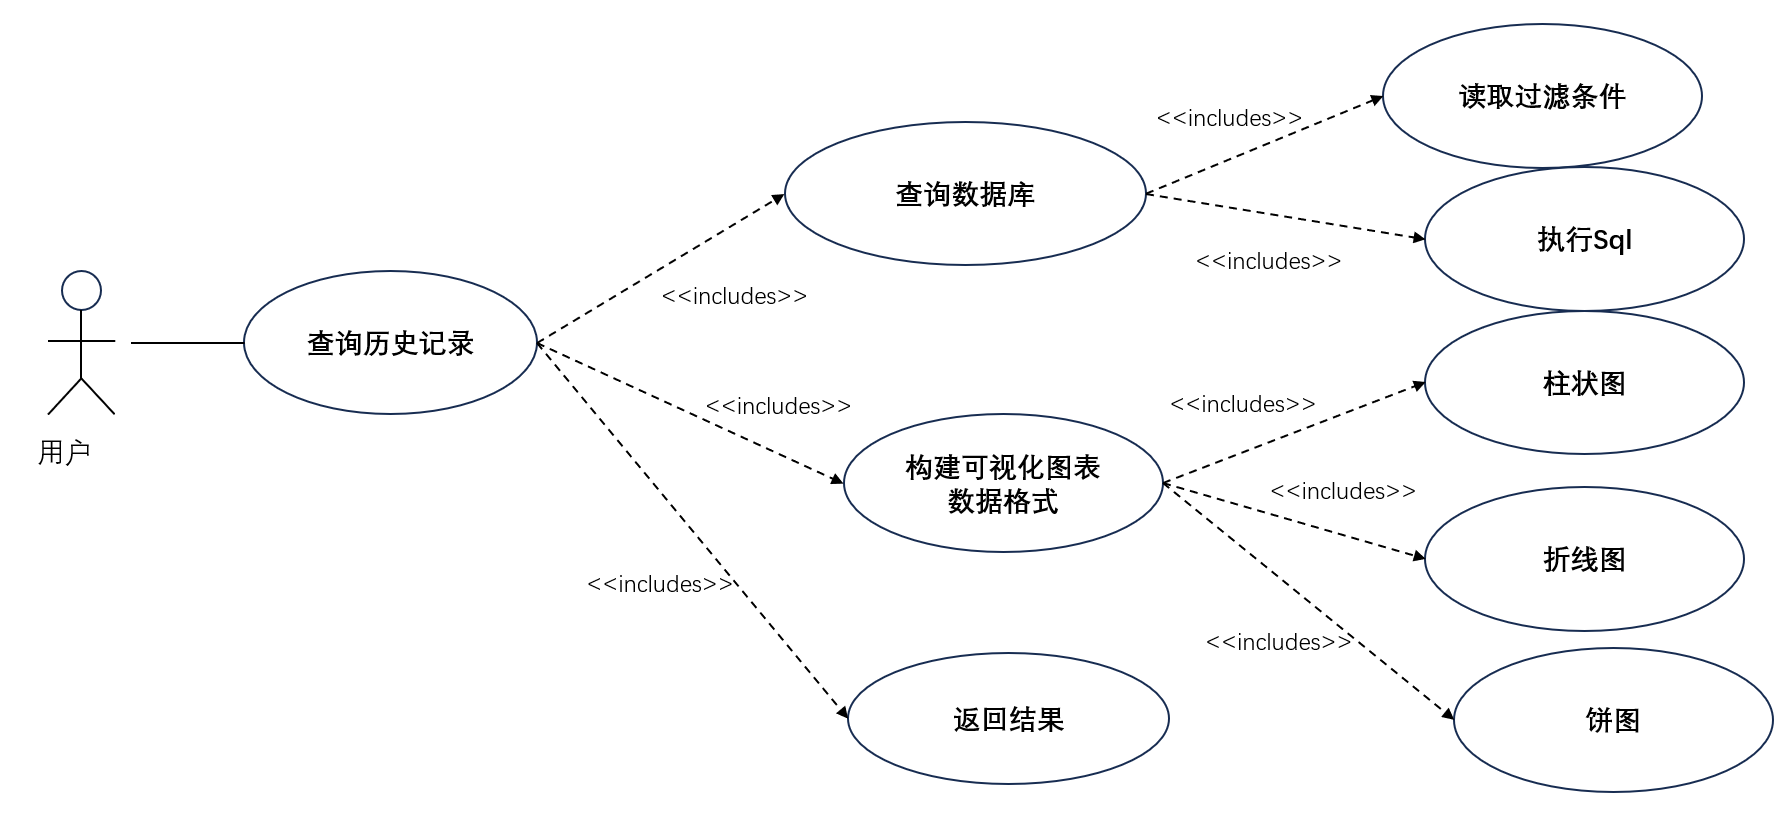
\includegraphics[width=0.95\textwidth]{figs/chap05/uml4.png}
    \caption{后端搜索模块用例图}
    \label{fig:uml4}
\end{figure}

\ref{fig:seq4}展示了后端搜索模块的操作顺序图。用户通过前端页面发起查询请求,该模块将过滤条件拼接到sql语句中去查询Mysql中的数据,根据ECharts文档执行数据格式转换操作,确保数据格式适配前端可视化图表。

\begin{figure}[h]
    \centering
    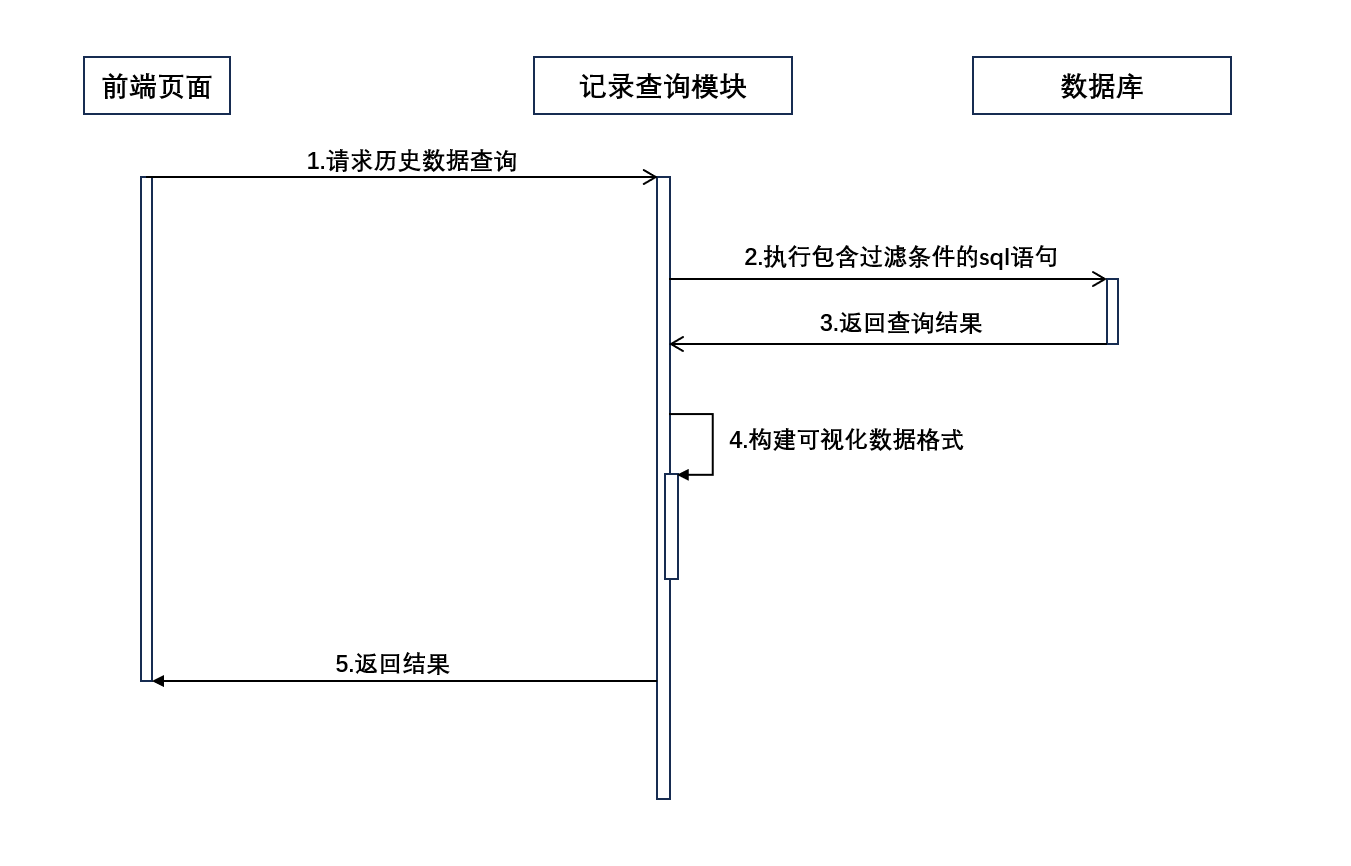
\includegraphics[width=0.95\textwidth]{figs/chap05/seq4.png}
    \caption{后端搜索模块顺序图}
    \label{fig:seq4}
\end{figure}

搜索模块的类图见\ref{fig:class2},包含SearchServiceImpl、SearchDTO和Detection三个类。SearchDTO作为search方法的输入参数,包含了用户自定义的过滤条件,包括对驾驶员、检测地点和检测时间这三个字段的过滤,对应用户在前端页面输入的过滤值。SearchServiceImpl的search方法负责根据过滤条件从数据库中搜索历史检测记录,用Detection类接收返回值。transform方法以查询出来的Detection结果集为输入,转换为可视化图表需要的特定数据格式。

\begin{figure}[h]
    \centering
    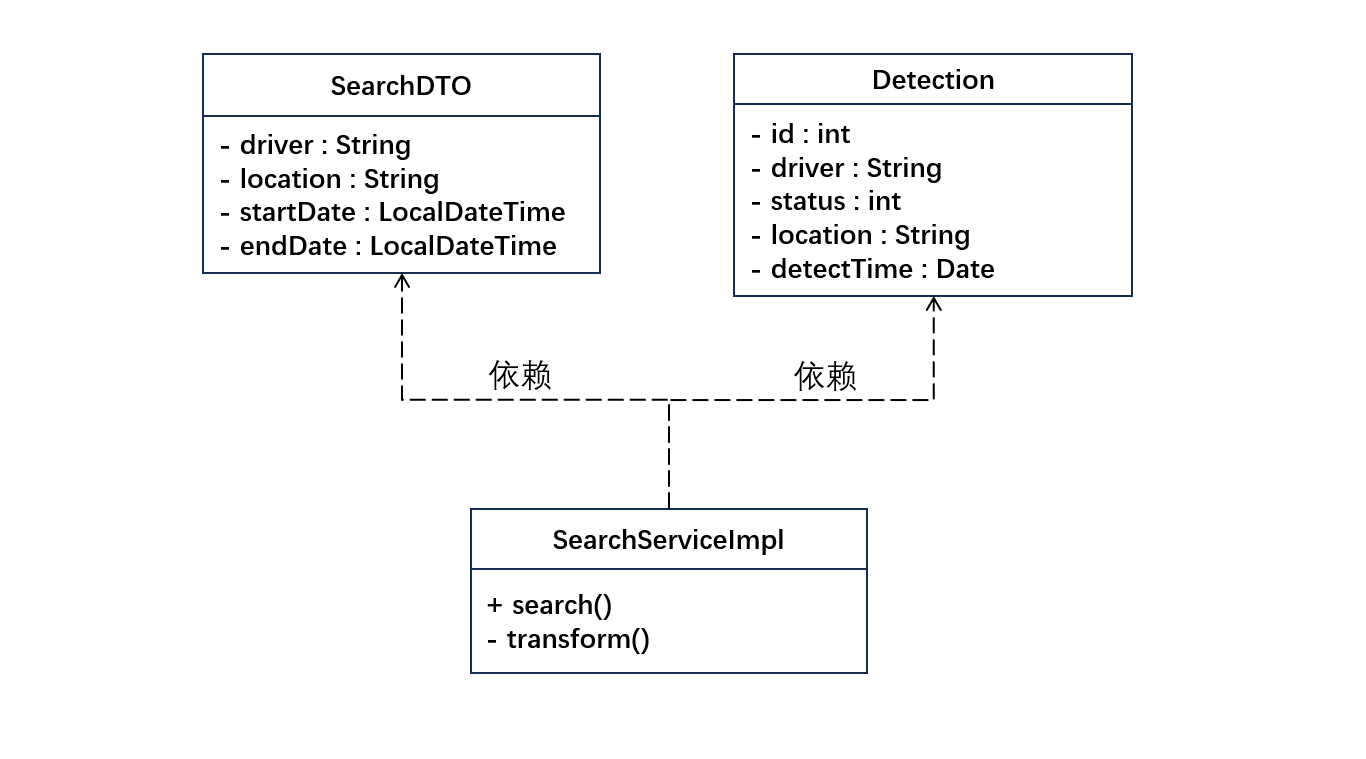
\includegraphics[width=0.9\textwidth]{figs/chap05/class2.png}
    \caption{后端搜索模块类图}
    \label{fig:class2}
\end{figure}

\section{本章小结}
本章首先对基于Vue和SpringBoot框架的摩托车驾乘人员头盔佩戴检测系统进行需求分析,然后通过用例图、顺序图和类图介绍了前端和后端各个模块的设计思路与具体实现。

